\subsection{Diagramy klas}

Zdecydowaliśmy się na wzorzec architektoniczny MVC (ang. Model View Controller). 
Jego zastosowanie umożliwia łatwą modyfikowalność, któregoś z komponentów, bez                                                                                               
konieczności zmian w pozostałych. Zgodnie z tym wzorcem w modelu zgromadzone są wszystkie dane naszego systemu. 
Widok odpowiada za prezentację aktualnego stanu systemu użytkownikowi, a kontroler odpowiada za zmianę modelu, a także odświeżanie widoków.
Na rysunku \ref{fig:mvc} przedstawiono trzy części wzorca MVC naszego systemu.

\begin{figure}[h]
    \centering
    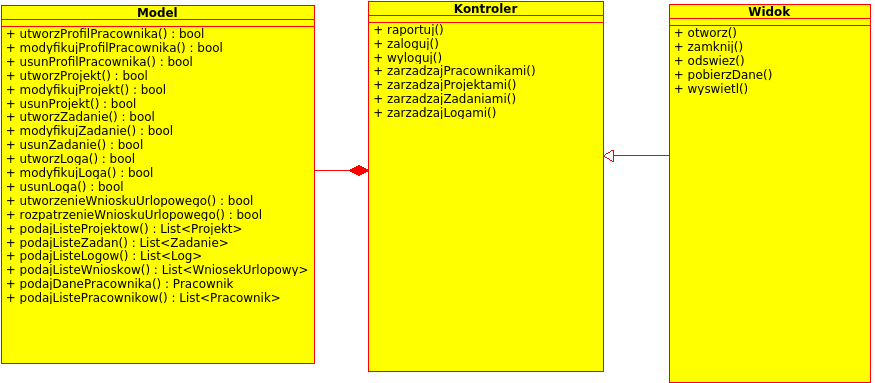
\includegraphics[scale=0.7]{modelKlas/mvc}
    \caption{Schemat architektury systemu zgodnej ze wzorcem architektonicznym MVC}
    \label{fig:mvc}
\end{figure}

Na rysunku \ref{fig:ModelDiagramKlas} przedstawiono szczegółowy diagram klas dla modelu. Projekt składa się z zadań składających się z logów, posiadających
treść. Każdy projekt ma kierownika projektu. Pracownik może złożyć wniosek urlopowy, a kadry się do niego ustosunkować (przyjąć bądź odrzucić).

\begin{figure}[h]
    \centering
    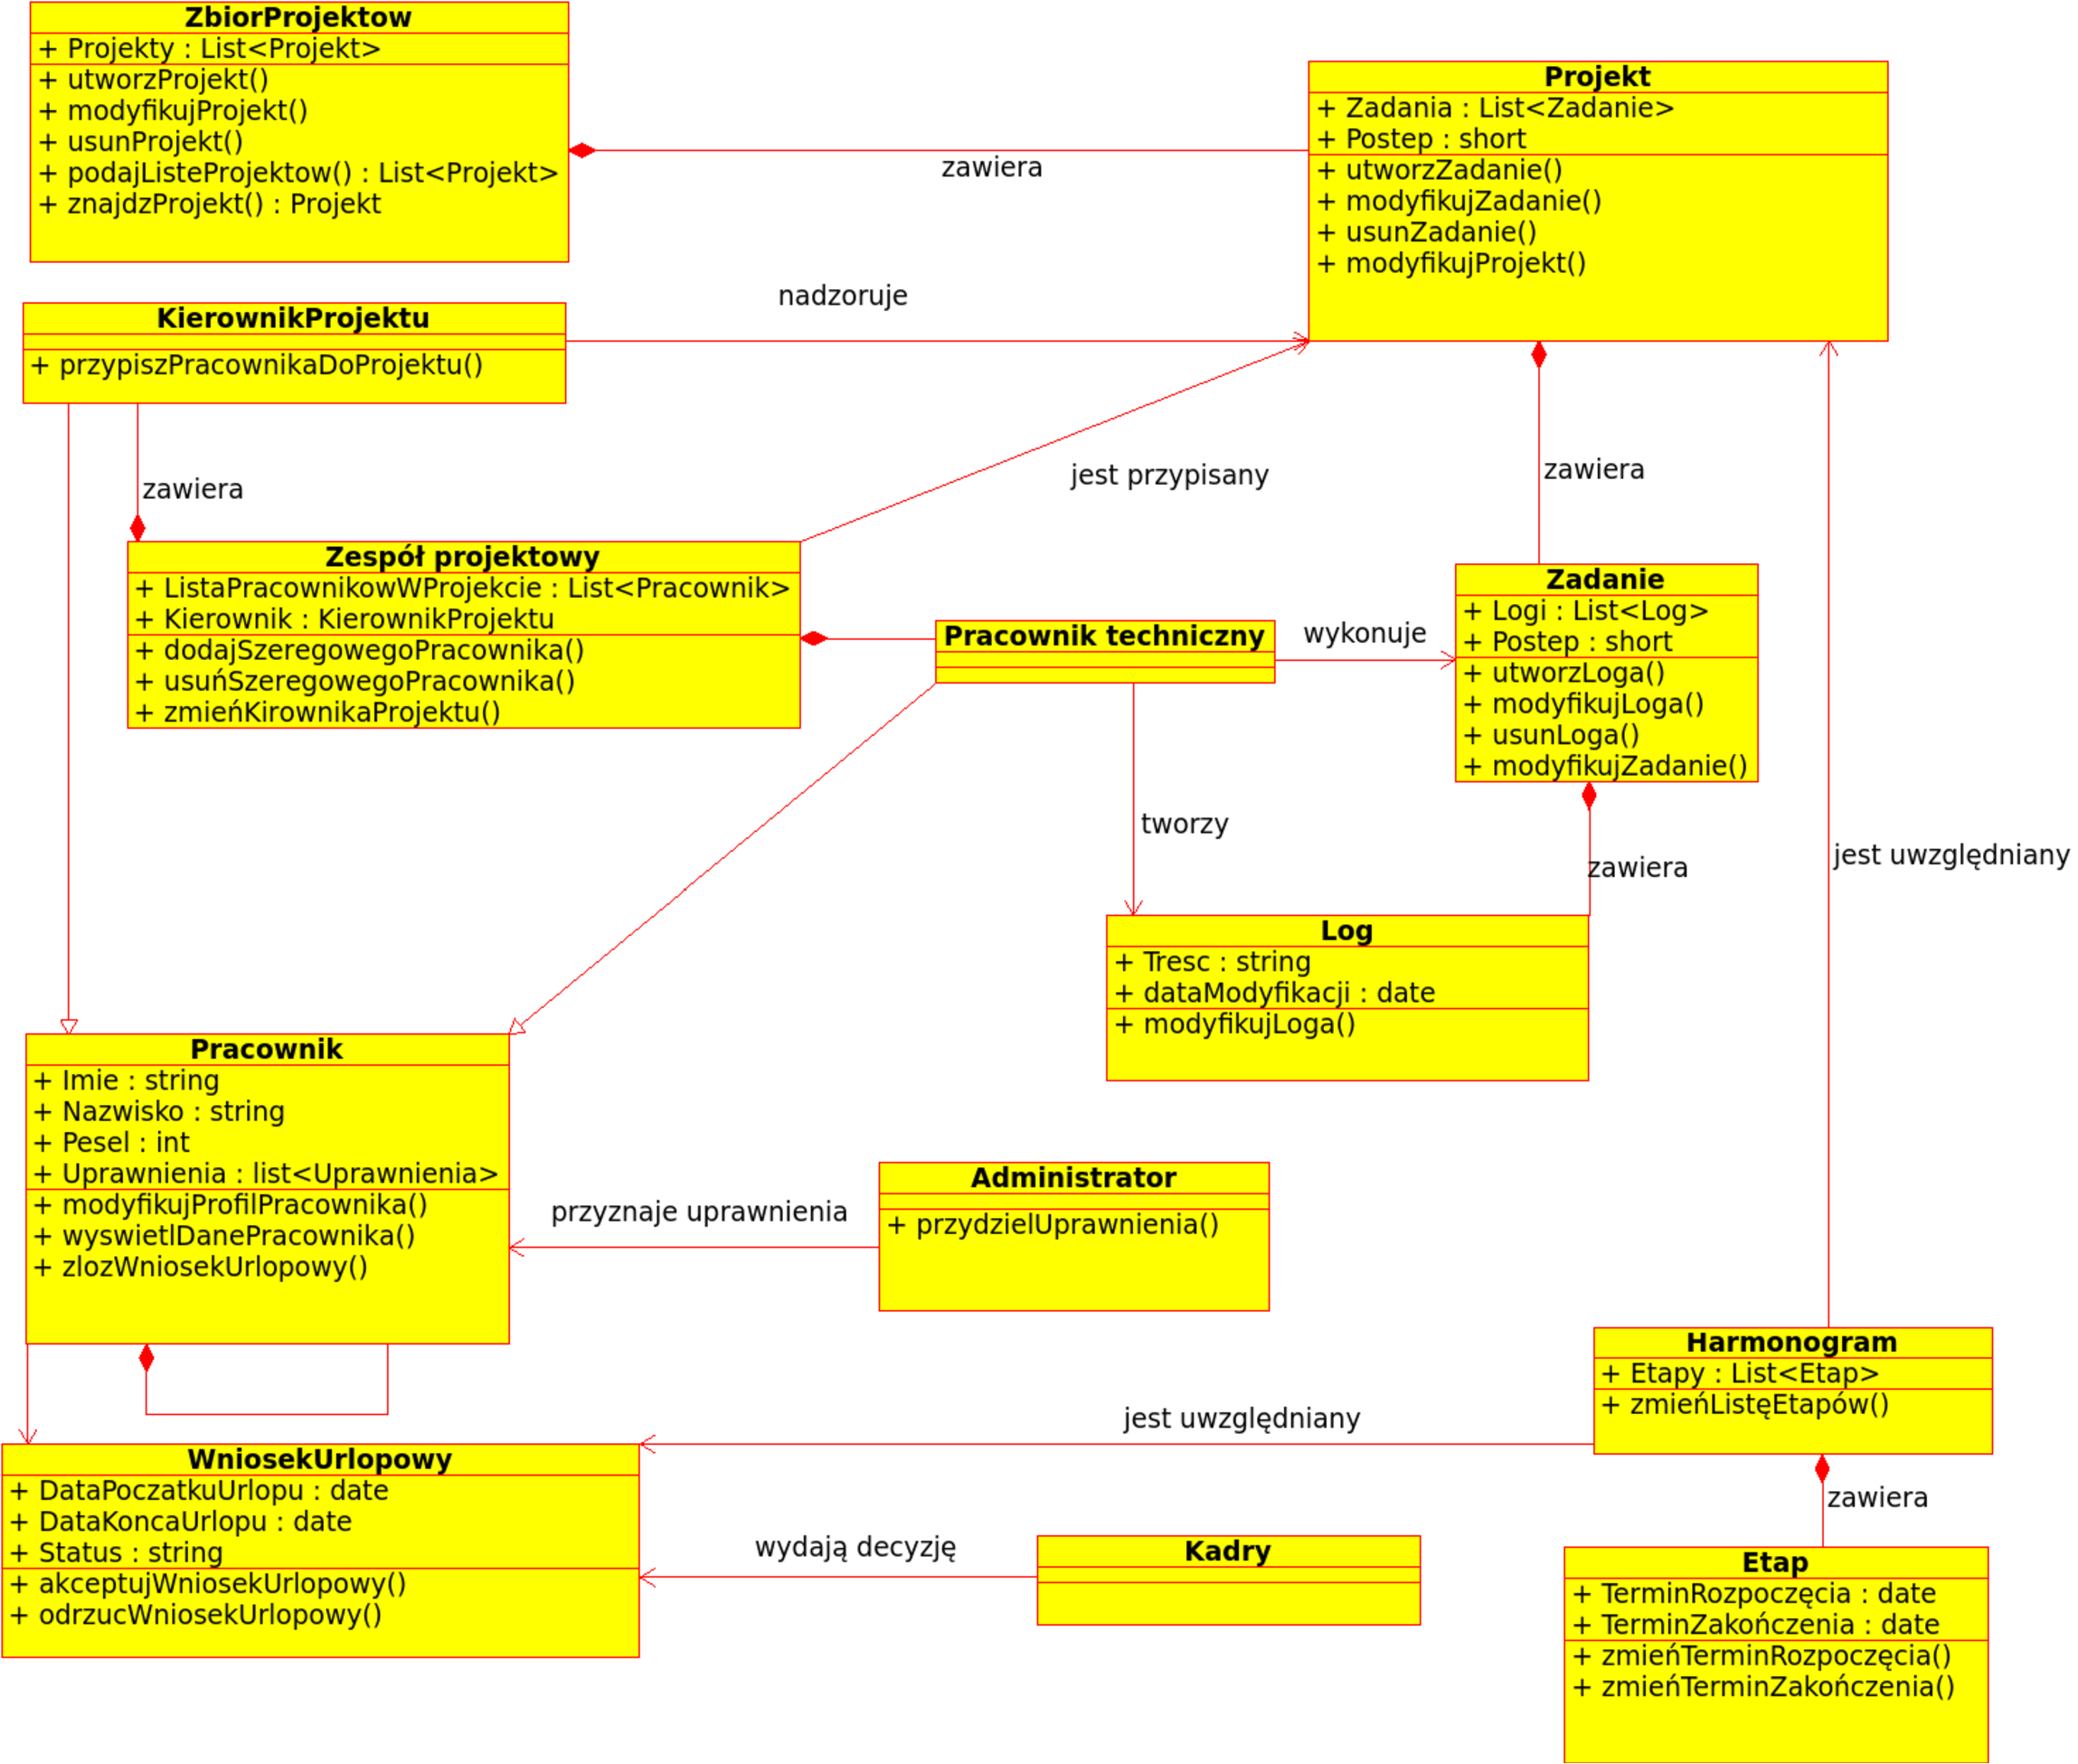
\includegraphics[scale=0.5]{modelKlas/ModelDiagramKlas}
    \caption{Diagram klas dla modelu.}
    \label{fig:ModelDiagramKlas}
\end{figure}

Rysunek \ref{fig:KontrolerDiagramKlas} prezentuje diagram klas dla kontrolera. Zadaniem kontrolera jest zarządzanie: pracownikami, projektmi, zadaniami i logami.

\begin{figure}[h]
    \centering
    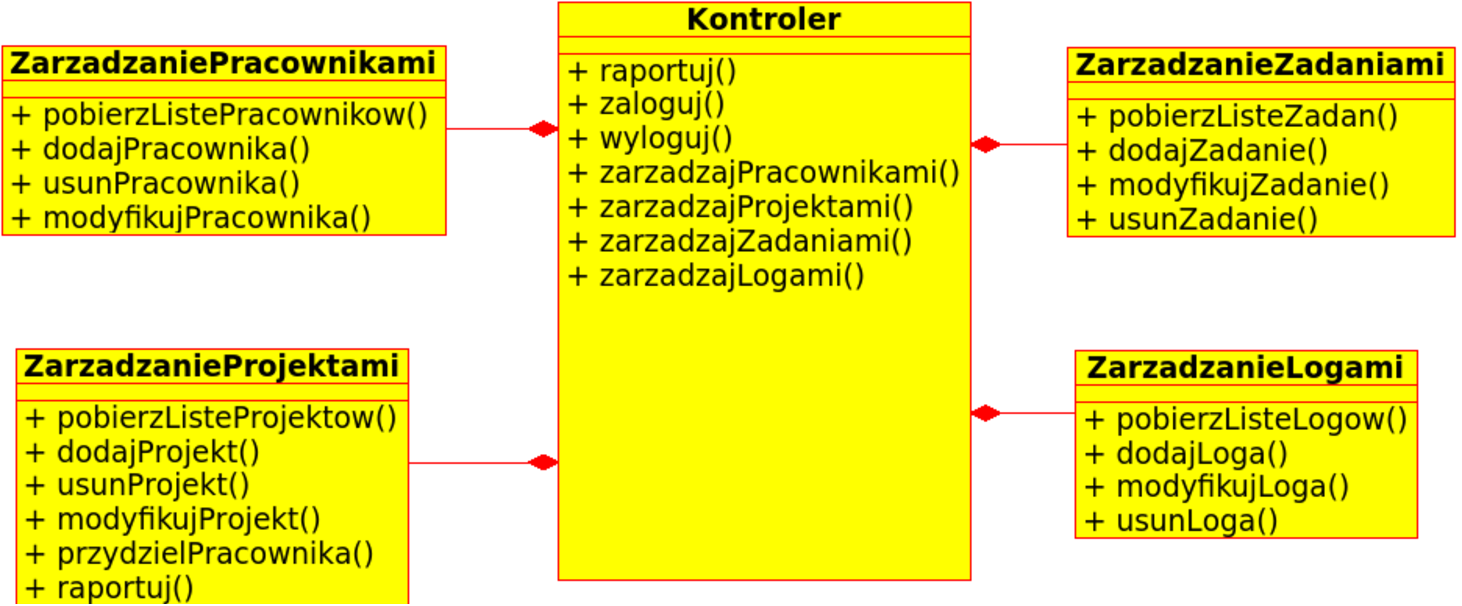
\includegraphics[scale=0.7]{modelKlas/KontrolerDiagramKlas}
    \caption{Diagram klas dla kontrolera.}
    \label{fig:KontrolerDiagramKlas}
\end{figure}

Rysunek \ref{fig:OknoDiagramKlas} przedstawia diagram klas dla okna. 
Okno jest odpowiedzialne za prezentowanie okien: logowania, raportu, zarządzania logami, zarządzania zadaniami, zarządzania projektami i pracownikami.


\begin{figure}[h]
    \centering
    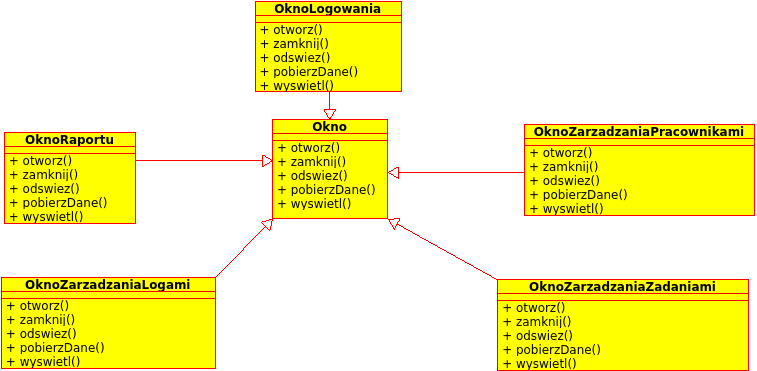
\includegraphics[scale=0.7]{modelKlas/OknoDiagramKlas}
    \caption{Diagram klas dla okna}
    \label{fig:OknoDiagramKlas}
\end{figure}

Zatwierdzanie loga przez kierownika projektu, opis relacji, dodac okno zarzadzania pracownikami
